% CVPR 2022 Paper Template
% based on the CVPR template provided by Ming-Ming Cheng (https://github.com/MCG-NKU/CVPR_Template)
% modified and extended by Stefan Roth (stefan.roth@NOSPAMtu-darmstadt.de)

\documentclass[10pt,twocolumn,letterpaper]{article}

%%%%%%%%% PAPER TYPE  - PLEASE UPDATE FOR FINAL VERSION
%\usepackage[review]{cvpr}      % To produce the REVIEW version
\usepackage{cvpr}              % To produce the CAMERA-READY version
%\usepackage[pagenumbers]{cvpr} % To force page numbers, e.g. for an arXiv version

% Include other packages here, before hyperref.
\usepackage{graphicx}
\usepackage{amsmath}
\usepackage{amssymb}
\usepackage{booktabs}

% It is strongly recommended to use hyperref, especially for the review version.
% hyperref with option pagebackref eases the reviewers' job.
% Please disable hyperref *only* if you encounter grave issues, e.g. with the
% file validation for the camera-ready version.
%
% If you comment hyperref and then uncomment it, you should delete
% ReviewTempalte.aux before re-running LaTeX.
% (Or just hit 'q' on the first LaTeX run, let it finish, and you
%  should be clear).
\usepackage[pagebackref,breaklinks,colorlinks]{hyperref}
\usepackage{multirow}


% Support for easy cross-referencing
\usepackage[capitalize]{cleveref}
\crefname{section}{Sec.}{Secs.}
\Crefname{section}{Section}{Sections}
\Crefname{table}{Table}{Tables}
\crefname{table}{Tab.}{Tabs.}


%%%%%%%%% PAPER ID  - PLEASE UPDATE
\def\cvprPaperID{*****} % *** Enter the CVPR Paper ID here
\def\confName{CVPR}
\def\confYear{2022}

\begin{document}

%%%%%%%%% TITLE - PLEASE UPDATE
\title{Open-Set Domain Adaptation through Self-Supervision}

\author{Protopapa Andrea, Quarta Matteo, Ruggeri Giuseppe, Versace Alessandro\\
Politecnico di Torino\\
Italy\\
{\tt\small \{s286302,s292477,s292459,s292477\}@studenti.polito.it <- Riordinare}
% For a paper whose authors are all at the same institution,
% omit the following lines up until the closing ``}''.
% Additional authors and addresses can be added with ``\and'',
% just like the second author.
% To save space, use either the email address or home page, not both
}
\maketitle

%%%%%%%%% ABSTRACT
\begin{abstract}
  Performance loss over domain change is a common problem in machine learning applications.
  Solving the issue usually relies on adapting the model to the new domain by having at disposal large and labeled datasets, either rare or costly to acquire.
  In this paper we propose a new approach, adapting models to the new domains while not needing relying on labeled data thanks to a self-supervision.
  Experiments conducted on the Office-Home dataset show interesting results and method effectiveness.
\end{abstract}

\section{Introduction}
\label{sec:intro}
Classical machine learning in the past years has made some oversimplified assumptions actually detached % Punteggiatura?
from the usage of artificial intelligence systems in everyday real world and the problems they come with.

The first assumption is that training and test sets come from the same distributions:
a model trained on labeled data is expected to perform as well as on the test data.
However, this assumption not always holds in real-world applications, 
where naively applying the trained model on a new dataset may cause degradation in the performance.
To solve this problem Domain Adaptation is widely used, 
where the goal is to train a neural network on a source dataset for which labels are available and search for good performance on a target dataset, 
which is related to but significantly different from the source dataset, 
and whose label or annotation is not available. 
Generally this is done by by minimizing the difference between domain distributions and enforcing the recognition of domain invariant patterns in both domains. 
As underlined in \cite{domainAdaptFarahani}, 
this is usually achieved by mapping source and target data by learning transformations for extracting such features and minimizing the gap between domains in the new representation space in an optimization procedure,
while preserving the underlying structure of the original data. 

Secondly, 
in real-world classification tasks it is usually difficult to collect training samples to exhaust all classes when training a model.
A more realistic scenario is open set recognition (OSR) \cite{OSRsurvey},
where incomplete knowledge of the world exists at training time and unknown classes can be injected during testing, 
requiring classifiers to not only accurately classify the seen classes but also effectively deal with unseen ones,
which would otherwise drastically weaken the robustness of the methods.
On the contrary this system should reject unknown classes at test time and separate the known and unknown samples.
As underlined by \cite{OSRclassRec}, 
existing open-set classifiers rely on deep networks trained in a supervised fashion on known classes in the training set;
this causes specialization of learned representations to known classes and makes it hard to distinguish the unknowns from the knowns.

To solve these significant issues our method is focused on a self-supervised task. 
Self-supervised learning is an unsupervised learning technique where the supervised task is created out of the unlabeled input data. 
This task could be as simple as predicting the lower half of an image being given the upper half of the same.
Supervised learning requires both labeled and high quality data,
usually very expensive, 
whereas unlabeled data is often readily available in abundance.
The fundamental idea behind self-supervised learning is creating some auxiliary task from input data so that,
by solving such task,
the model can learn the underlying structure of the data,
for instance high-level knowledge, correlations, and metadata embedded in the data.
This type of learning was recently used for Domain Adaptation, 
learning robust cross-domain features and supporting generalization \cite{CarlucciJigsaw,SelfSupervisedXu},
and also for some Open Set problems specialized in anomaly detection and discriminating anomalous data \cite{bergman2020classificationbased,dectionGeometric}.

The approach presented in this paper brings these topics together in the so called Open-Set Domain Adaptation (OSDA) problem. 
A two-stage method is hence proposed, 
aiming to identify and isolate unknown class samples in the first stage, 
before reducing in the second stage the domain gap between the source domain and the known target domain to avoid negative transfer.
This is done in both stages using a modified version of the rotation task as self-supervised model,
predicting the relative rotation between an image and its rotated version.
Finally a classifier is used to predict if each target sample belongs either to one of the knwon classes or to an unknown class, 
being rejected in the latter case.

The method was evaluated on the Office-Home benchmark \cite{OfficeHomeDataset} with a specific OSDA metric.

{\bf ADD HERE RESULTS AND A BRIEF OF CONCLUSIVE IDEAS (ALSO POSSIBLE FUTURE WORKS)!!}

%------------------------------------------------------------------------
\section{Related Work}
\label{sec:relatedwork}


\section{Method}
\label{sec:method}

\subsection{Problem Formulation}
\label{sec:problemformulation}
Our starting point is the source dataset, 
defined as $\mathcal{D}_s = \{({\bf x}_i^s, y_i^s)\}_{i=1}^{N_S} \sim p_s$, 
where each element ${\bf x}_i^s$ belonging to class $y_i^s$ is a sample from the source domain {\it S}.
This dataset has a target counterpart, 
$\mathcal{D}_t = \{{\bf x}_i^t\}_{i=1}^{N_t} \sim p_t$ which is unlabeled instead.
In OSDA we have that $p_s \neq p_t$.
The source dataset $\mathcal{D}_s$ is associated with a set of known classes $\mathcal{C}_s$, 
which can also be found in the target dataset $\mathcal{D}_t$ but is supposedly smaller.
In other words,
$|\mathcal{C}_s| < |\mathcal{C}_t|$ and $\mathcal{C}_s \subset \mathcal{C}_t$.
In domain adaptation, 
we further have that the target distribution of the known source classes differs from the target distribution of known classes,
so $p_t^s \neq p_s$, 
A metric to measure how different two domains are is the openness betweeen source and target domain\cite{bendale2015open}, 
defined as $\displaystyle \mathbb{O} = 1-\frac{\mathcal{C}_s}{\mathcal{C}_t}$.
When $\mathbb{O} > 0$, we're dealing with an OSDA problem.

\subsection{Approach}
\label{sec:apporach}
The task is split in two separate stages.
First, 
we have to train the model to separate between the known classes ($\mathcal{C}_s$) and the unknown classes ($\mathcal{C}_{t\setminus s})$ in a reliable way.
This is achieved via the self-supervised task,
training the model to both recognize the class of a sample and its relative orientation.
Secondly,
we train the model on a union of both source and target datasets,
to reject samples when they are not part of the known classes $\mathcal{C}_s$.

\subsection{Rotation Recognition}

We denote with $rot({\bf x}, k)$ the rotation of the sample image {\bf x} by $k\times 90$ degrees clockwise.
This is the self-supervised part of our proposed model as rotation indices $k \in [0, 3]$ can be randomly generated and then predicted.
Relative rotation,
meaning that both original and rotated features are supplied to the model,
is preferred over just using rotated features as some objects might not have an absolute correct orientation.
Alternatively, 
instead of having the model predict the rotation of a sample for any class using the same classifier, 
we also try using a different head for each one of the known classes $\mathcal{C}_s$.

\subsection{Step I: Sample Separation}

Separating samples requires iterating over $\tilde{\mathcal{D}_s} = \{({\bf x}_i^s, {\bf \tilde x}_i^s, z_i^s)\}_{i=1}^{N_s}$,
where ${\bf \tilde x}_i^s$ is the $z_i^s\times 90$ degrees rotated version of ${\bf x}_i^s$.
The network is composed by an extractor $E$ and two classifiers, 
$R_1$ and $C_1$.
$C_1$ is the object classifier, 
assigning image labes $\tilde{y}_i^s \in \{0, \dots, |\mathcal{C}_s|\}$,
while $R_1$ is the relative rotation classifier,
assigning rotation indices $\tilde{z}_i^s \in [0, 3]$.
${\bf\tilde{z}}_i^s$ and ${\bf\tilde{y}}_i^s$ are the vector representations of $\tilde{z}_i^s$ and $\tilde{y}_i^s$.
The multi-head rotation classifier uses $|\mathcal{C}_s|$ heads for the rotation task.
In this case, 
which head to use during separation is up to the object classifier $C_1$.
Object predictions are made as ${\bf\tilde{x}}_i^s = softmax(E({\bf x}_i^s))$,
while relative rotation predictions are computed as ${\bf \tilde z}_s = softmax(R_1([E({\bf x}^s), E({\bf\tilde x}^s)]))$.
If a multi-head rotation classifier is used,
the $j = y_i^s$ head is used as ${\bf\tilde{z}}_s = softmax(R_{1,j}[E({\bf x}^s), E({\bf\tilde{x}}^s)])$.
The model is trained to minimizing the objective function $\mathcal{L}_1 = \mathcal{L}_{C_1} + \mathcal{L}_{R_1}$.
This is the sum of two cross-entropy loss functions:

\begin{equation}
  \mathcal{L}_{C_1} = -\sum_{i\in\mathcal{D}_s} {\bf y}_i^s \log \tilde{\bf y}_i^s
  \label{eq:baseloss_class}
\end{equation}

\begin{equation}
  \mathcal{L}_{R_1} = -\alpha_1\sum_{i\in\mathcal{\tilde{D}}_s} {\bf y}_i^s \log \tilde{{\bf z}}_i^s
  \label{eq:baseloss_rot}
\end{equation}

Where $\alpha_1$ is a weight associated to the rotation task.
We also try using an extended rotation loss function $\mathcal{L}_{R_1}^*$ implementing an additional center loss\cite{CenterLoss} term:

\begin{equation}
  \mathcal{L}_{R_1}^* = -\alpha_1\sum_{i\in\mathcal{D}_s} {\bf y}_i^s \log \tilde{{\bf z}}_i^s+\lambda_1||{\bf v}_i^s-\gamma({\bf z}_i^s)||_2^2
  \label{eq:center_loss}
\end{equation}

Here ${\bf v_i}$ is the penultimate layer of the rotation classifier,
called features, 
$\gamma({\bf z}_i)$ is the center of the features associated to class $i$,
$||\cdot||_2^2$ is the $l$-2 norm and $\lambda_1$ is the weight associated with the center loss term.

When training is completed, 
we can start separating samples.
To do so,
normality scores $\mathcal{N}(\cdot)$ are used,
defined as the maximum prediction of the rotation classifier:
$\mathcal{N}({\bf\tilde{x}}_i) = \max({\bf\tilde{z}}_i)$.
To predict wheter a sample belongs to the known samples of the target domain $\mathcal{D}_t^{knw}$ or the unknown ones $\mathcal{D}_t^{unk}$ requires picking a threshold $\tilde{\mathcal{N}}$.
The separation is then done as:

\begin{equation}
  \begin{cases}
    {\bf x}_i^t \in \mathcal{D}_t^{knw} & \text{ if } \mathcal{N}({\bf\tilde x}_i^t) \geq \tilde{\mathcal{N}} \\
    {\bf x}_i^t \in \mathcal{D}_t^{unk} & \text{ if } \mathcal{N}({\bf\tilde x}_i^t) < \tilde{\mathcal{N}}
  \end{cases}
  \label{eq:sample_separation}
\end{equation}

When using a multi-head rotation classifier, 
it is required to choose among the $|\mathcal{C}_s|$ possible heads to make the prediction.
Head $R_{1,j}$ is used by choosing $j$ as $\displaystyle j = \arg\max_j {\bf\tilde{y}}_i^t$.

\subsection{Step II: Domain Alignment}
\label{sec:domain_alignment}

\begin{figure*}
  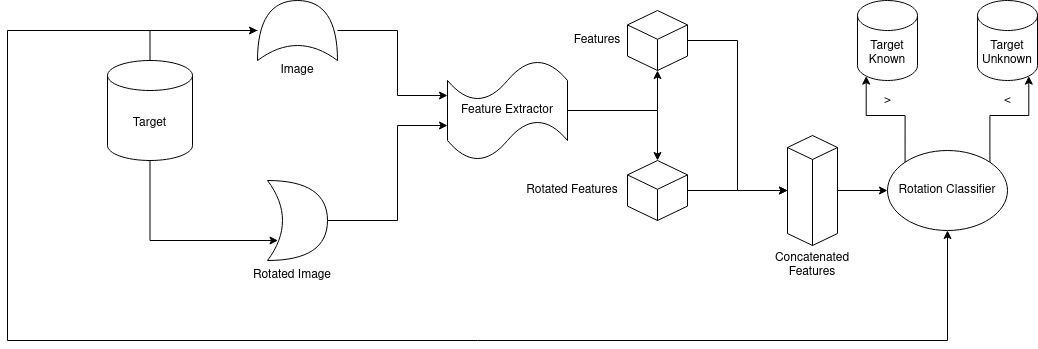
\includegraphics[width=\textwidth ]{scheme.png}
  \caption{\label{fig:separation} Schema representing the target images separation process}
\end{figure*}

In this phase,
we build two "new" datasets.
The first one is $\mathcal{D}_s^*$, composed as $\mathcal{D}_s \cup \mathcal{D}_t^{unk}$.
Since $\mathcal{D}_t$ is an unlabeled dataset but $\mathcal{D}_s^*$ is a labeled one,
samples in $\mathcal{D}_t^{unk}$ are labeled as unknowns.
The second one is $\mathcal{D}_t^{knw}$.
Here we also use two new classifiers,
$C_2$ and $R_2$,
similarly to how they were used in the first phase but with $C_2$ predicting $|\mathcal{C}_s|+1$ classes to accomodate unknown predictions.
In this step $R_2$ is always single-headed and has its own weight $\alpha_2$.
The objective function is the same described in equations \ref{eq:baseloss_class} and \ref{eq:baseloss_rot}.
The main difference here is that $C_2$ is actually trained to recognize unknown classes,
on both domains.

\subsection{Performance Metrics}
\label{sec:performance_metrics}

Evaluating model perfomance requires finding a balance between two values:
{\it OS*}, 
the fraction of correctly classified samples,
and {\it UNK}, 
the fraction of correclty rejected samples.
A model not confident enough to reject a sample could still achieve high {\it OS*} values but near-zero {\it UNK},
while a model rejecting every  sample as unkwnown will achieve perfect {\it UNK} and zero {\it OS*}.
To compare models we use the harmonic mean between {\it OS*} and {\it UNK}, 
defined as $HOS = 2\frac{OS^*\times UNK}{OS^*+UNK}$.
This is because this kind of mean tends gives a bigger weight to the smaller values,
resulting in a more severe evaluation of models.

\section{Experiments}
\label{sec:experiments}

\subsection{Dataset}
\label{sec:dataset}

Our model is tested on the {\it Office-Home} dataset\cite{OfficeHomeDataset}, 
which features 65 classes of images over four different domains: Art (A), Clipart (C), Product (P) and Real World (R).
We set the first 45 classes to be known while the remaining 20 are unknown.
For each experiment, 
we report both the best achieved HOS as well as the last reported HOS.
As separation is crucial for the model effectiveness,
 we also report the computer AUROC score for the first part.

\subsection{Results}
\label{sec:results}
Table \ref{tab:results} contains the results for all 12 {\bf (ne abbiamo provati davvero 12???)} available domain shifts,
as well as perfomance differences when using multi-head rotation classifiers and center loss.
Further details are to be found in section \ref{sec:implementation_details}.
We can notice that multi-headed models are more capable of correctly discriminating between known and unknown samples,
ultimately resulting in better domain alignment.
A further advantage is given when combined with center loss.
AUROC values are computed at the end of the separation stage, 
while HOS values are sampled at regular times on the entire original target dataset.


\begin{table}
  \centering
  \begin{tabular}[t]{||c|c|c||c|c||}
    \hline
    \multicolumn{5}{||c||}{Single-Head, CE Loss} \\
    \hline
    Source & Target & AUROC & HOS & HOS* \\
    S & T & 50\% & 30\% & 30\% \\
    S & T & 50\% & 30\% & 30\% \\
    S & T & 50\% & 30\% & 30\% \\
    \hline
    \hline
    \multicolumn{5}{||c||}{Multi-Head, CE Loss} \\
    \hline
    Source & Target & AUROC & HOS & HOS* \\
    S & T & 50\% & 30\% & 30\% \\
    S & T & 50\% & 30\% & 30\% \\
    S & T & 50\% & 30\% & 30\% \\
    \hline
    \hline
    \multicolumn{5}{||c||}{Single-Head, CE+C Loss} \\
    \hline
    Source & Target & AUROC & HOS & HOS* \\
    S & T & 50\% & 30\% & 30\% \\
    S & T & 50\% & 30\% & 30\% \\
    S & T & 50\% & 30\% & 30\% \\
    \hline
    \hline
    \multicolumn{5}{||c||}{Multi-Head, CE+C Loss} \\
    \hline
    Source & Target & AUROC & HOS & HOS* \\
    S & T & 50\% & 30\% & 30\% \\
    S & T & 50\% & 30\% & 30\% \\
    S & T & 50\% & 30\% & 30\% \\
    \hline 
    \hline
    \multicolumn{5}{||c||}{No Rotation} \\
    \hline
    Source & Target & AUROC & HOS & HOS$_{Best}$ \\
    S & T & 50\% & 30\% & 30\% \\
    S & T & 50\% & 30\% & 30\% \\
    S & T & 50\% & 30\% & 30\% \\
    \hline
  \end{tabular}
  \caption{\centering\label{tab:results}Results for domain alignment. AUROC is the area under the ROC. HOS is latest achieved HOS, HOS* the best achieved through all epochs.}
\end{table}

\section{Implementation Details}
\label{sec:implementation_details}
\subsection{Model Parameters}
\label{sec:model_parameters}

All models were run using stochastic gradient descent with batch size 32,
a weight decay of 0.0005 and momentum of 0.9.
For single-headed models, 
a base learning rate of 0.001 is used,
while for multi-headed models it is set to 0.003.
This is because only one head of the heads is trained with each samples,
so the process needs to be sped up.
Rotation classifier use a learning rate set to a tenth of the base learning rate.
A step learning rate scheduler is used, reducing it by a factor of 10 after 90\% of epochs.
All models are run for 50 epochs for the first step described in \ref{eq:sample_separation} and for 25 epochs for the second step described in \ref{sec:domain_alignment}.
For model using the center loss a centroid learning rate of 0.5 is used.
All other parameters are configuration-sepcific and are reported in table \ref{tab:params}.
"No Rotation" model is the same as a single-head without center loss model with $\alpha_2 = 0$.


% % % 

{\it Extractor E}: The extractor employed is a ResNet-34{\bf[Inserire cit a ResNet]} {\bf è pretrained???} {\bf ma 34 o 18???} for all classifiers.

{\it Classifier $C_1$, $C_2$}: $C_1$ is composed of a 45 dimensional output. 
All unknown samples are mapped as belonging to class 45.
$C_1$ is used as a starting point for $C_2$.
As no unknowns are present on the source dataset (they are removed),
the weight of unknwon samples in the second step is set to {\bf spiegare come è bilanciato} while for all other classes it is set to 1.
A single fully connected layer $512\to 45$ with batch-norm is used.

{\it Classifier $R_1$, $R_2$}: 
$R_1$ and $R_2$ are composed by a $1024\to 256$  and a $256\to 4$ fully connected layers, named {\it Discriminators}.
The 256-dimensional output are the features used by the center loss for inferring class centers.
If multi-head is used, each head is a separate discriminator.
$R_2$ is always a single-head classifier, even if using a multi-head rotation classifier.



\begin{table}
  \centering
  \begin{tabular}[b]{||c|c|c|c|c|c||}
    \hline
    MH & CL & $\alpha_1$ & $\alpha_2$ & $\lambda_1$ & $\mathcal{\tilde N}$ \\
    \hline
    Off & Off & 0.0 & 0.0 & 0.0 & 0.0 \\
    On & Off & 0.0 & 0.0 & 0.0 & 0.0 \\
    Off & On & 0.0 & 0.0 & 0.0 & 0.0 \\
    On & On & 0.0 & 0.0 & 0.0 & 0.0 \\
    \hline
  \end{tabular}
  \caption{\label{tab:params}Model Parameters}
\end{table}

\subsection{Ablation Study}
\label{sec:ablation_study}
As shown in table \ref{tab:results} different architectures give different results, 
and as shown in table \ref{tab:params} each one requires a different set of parameters.
To choose optimal parameters a sequential approach is followed, 
by optimizing one parameter at the time.
The order of optimization followed is: 
$\alpha_1$, $\lambda_1$, $\mathcal{\tilde N}$, $\alpha_2$.
Models not using center loss just skip the $\lambda_1$ optimization.
Ablation study were run on two domain shifts, 
Art $\to$ Clipart and Clipart $\to$ Product.
In table \ref{tab:ablation_params} we report the steps followed.
All other settings follow what is reported in \ref{sec:model_parameters}.
The result here obtained are the same reported in table \ref{tab:params}.


\begin{table}
  \centering
  \begin{tabular}[h]{||c|c|c||c|c||}
    \hline
    \multicolumn{5}{||c||}{MH OFF CL OFF} \\
    \hline
    $\alpha_1$ & $\mathcal{\tilde N}$ & $\alpha_2$  & AUROC & HOS$_{mean}$\\    
    \hline
    \hline
    \multicolumn{5}{||c||}{Picking $\alpha_1$} \\
    \hline
    1.0 & \multirow{4}{*}{0.5} & \multirow{4}{*}{3.0} & 0.5 & 30\% \\
    3.0 & & & 0.5 & 30\% \\
    5.0 & & & 0.5 & 30\% \\
    10.0 & & & 0.5 & 30\% \\
    \hline
    \hline
    \multicolumn{5}{||c||}{Picking $\mathcal{\tilde N}$} \\
    \hline
    \multirow{4}{*}{1.0} & 0.40 & \multirow{4}{*}{3.0} & 0.5 & 50\%\\
    & 0.50 && 0.5 & 50\% \\
    & 0.55 && 0.5 & 50\% \\
    & 0.60 && 0.5 & 50\% \\
    \hline
    \hline
    \multicolumn{5}{||c||}{Picking $\alpha_2$} \\
    \hline
    \multirow{4}{*}{1.0} & \multirow{4}{*}{0.6} & 1.0 & 0.5 & 50\%\\
    && 3.0 & 0.5 & 50\% \\
    && 5.0 & 0.5 & 50\% \\
    && 10.0 & 0.5 & 50\% \\
    \hline
    \hline
    \multicolumn{5}{||c||}{Final Parameters} \\
    \hline
    1.0 & 0.6 & 3.0 & 0.5 & 50\%\\
    \hline
  \end{tabular}
  \caption{\label{tab:ablationoffoff} Ablation performed for OFF-OFF configuration}
\end{table}
\section{Future Work}

The results show that self-supervision technique can help in domain adaptation task and open-set classification tasks.
A few critical points still remain on our method of study and proposed solution.
The most important one is probably parameter choosing for different models, as we have seen that variations cause huge differences in results and sequential optimization of parameter is a sub-optimal heuristic.
Furthermore, having the model to learn two different tasks at once, it could be useful to use a slower learning model at the expense of longer training times.

%%%%%%%%% REFERENCES
{\small
\bibliographystyle{ieee_fullname}
\bibliography{egbib}
}

\end{document}
